\documentclass{article}

\usepackage[T2A]{fontenc}
\usepackage[utf8]{inputenc}
\usepackage[english, russian]{babel}
\usepackage[a4paper, margin=1in]{geometry}
\usepackage{graphicx}
\usepackage{amsmath}
\usepackage{mathtools}
\usepackage{pgfplots}
\usepackage{pgfplotstable}
\usepackage{setspace}
\usepackage{changepage}
\usepackage{caption}
\usepackage{csquotes}
\usepackage{hyperref}
\usepackage{listings}

\pgfplotsset{compat=1.18}

\definecolor{codegreen}{rgb}{0,0.6,0}
\definecolor{codegray}{rgb}{0.5,0.5,0.5}
\definecolor{codepurple}{rgb}{0.58,0,0.82}
\definecolor{backcolour}{rgb}{0.99,0.99,0.99}

\lstdefinestyle{codestyle}{
  backgroundcolor   = \color{backcolour},
  commentstyle      = \color{codegreen},
  keywordstyle      = \color{magenta},
  numberstyle       = \tiny\color{codegray},
  stringstyle       = \color{codepurple},
  basicstyle        = \ttfamily\footnotesize,
  breakatwhitespace = false,
  breaklines        = true,
  captionpos        = b,
  keepspaces        = true,
  numbers           = left,
  numbersep         = 5pt,
  showspaces        = false,
  showstringspaces  = false,
  showtabs          = false,
  tabsize           = 2
}

\lstset{
    basicstyle=\ttfamily,
    inputencoding=utf8,
    extendedchars=true,
    literate={а}{{\selectfont\char224}}1
             {б}{{\selectfont\char225}}1
             {в}{{\selectfont\char226}}1
             {г}{{\selectfont\char227}}1
             {д}{{\selectfont\char228}}1
             {е}{{\selectfont\char229}}1
             {ё}{{\"e}}1
             {ж}{{\selectfont\char230}}1
             {з}{{\selectfont\char231}}1
             {и}{{\selectfont\char232}}1
             {й}{{\selectfont\char233}}1
             {к}{{\selectfont\char234}}1
             {л}{{\selectfont\char235}}1
             {м}{{\selectfont\char236}}1
             {н}{{\selectfont\char237}}1
             {о}{{\selectfont\char238}}1
             {п}{{\selectfont\char239}}1
             {р}{{\selectfont\char240}}1
             {с}{{\selectfont\char241}}1
             {т}{{\selectfont\char242}}1
             {у}{{\selectfont\char243}}1
             {ф}{{\selectfont\char244}}1
             {х}{{\selectfont\char245}}1
             {ц}{{\selectfont\char246}}1
             {ч}{{\selectfont\char247}}1
             {ш}{{\selectfont\char248}}1
             {щ}{{\selectfont\char249}}1
             {ъ}{{\selectfont\char250}}1
             {ы}{{\selectfont\char251}}1
             {ь}{{\selectfont\char252}}1
             {э}{{\selectfont\char253}}1
             {ю}{{\selectfont\char254}}1
             {я}{{\selectfont\char255}}1
             {А}{{\selectfont\char192}}1
             {Б}{{\selectfont\char193}}1
             {В}{{\selectfont\char194}}1
             {Г}{{\selectfont\char195}}1
             {Д}{{\selectfont\char196}}1
             {Е}{{\selectfont\char197}}1
             {Ё}{{\"E}}1
             {Ж}{{\selectfont\char198}}1
             {З}{{\selectfont\char199}}1
             {И}{{\selectfont\char200}}1
             {Й}{{\selectfont\char201}}1
             {К}{{\selectfont\char202}}1
             {Л}{{\selectfont\char203}}1
             {М}{{\selectfont\char204}}1
             {Н}{{\selectfont\char205}}1
             {О}{{\selectfont\char206}}1
             {П}{{\selectfont\char207}}1
             {Р}{{\selectfont\char208}}1
             {С}{{\selectfont\char209}}1
             {Т}{{\selectfont\char210}}1
             {У}{{\selectfont\char211}}1
             {Ф}{{\selectfont\char212}}1
             {Х}{{\selectfont\char213}}1
             {Ц}{{\selectfont\char214}}1
             {Ч}{{\selectfont\char215}}1
             {Ш}{{\selectfont\char216}}1
             {Щ}{{\selectfont\char217}}1
             {Ъ}{{\selectfont\char218}}1
             {Ы}{{\selectfont\char219}}1
             {Ь}{{\selectfont\char220}}1
             {Э}{{\selectfont\char221}}1
             {Ю}{{\selectfont\char222}}1
             {Я}{{\selectfont\char223}}1
}

\lstset{style=codestyle}

\graphicspath{{../figure/}}

\hypersetup{
  colorlinks = true,
  linkcolor  = blue,
  filecolor  = magenta,
  urlcolor   = darkgray,
  pdftitle   = P34131 Смирнов В. И. и Черемнов К. Д.,
}

\begin{document}

\begin{titlepage}
  \begin{center}
    \begin{spacing}{1.4}
      \large{Университет ИТМО} \\
      \large{Факультет программной инженерии и компьютерной техники} \\
    \end{spacing}
    \vfill{}
    \textbf{
      \huge{Моделирование} \\
      \huge{Учебно-исследовательская работа №4} \\
      \huge{Исследование сетевых моделей массового обслуживания} \\
    }
  \end{center}
  \vfill{}
  \begin{center}
    \begin{tabular}{r l}
      Группа:        & P34131                         \\
      Студент 1:     & Черемнов Константин Дмитриевич \\
      Студент 2:     & Смирнов Виктор Игоревич        \\
      Вариант        & 14/3                           \\
      Преподаватель: & Тропченко Андрей Александрович \\
    \end{tabular}
  \end{center}
  \vfill{}
  \begin{center}
    \begin{large}
      2024
    \end{large}
  \end{center}
\end{titlepage}

\section*{Ключевые слова}

Моделирование, СМО, Замкнутые и разомкнутые СМО, СеМО

\tableofcontents

\section{Цель работы}

Исследование свойств системы, моделируемой в виде замкнутых и разомкнутых сетей массового обслуживания (СеМО) с однородным потоком заявок с применением имитационного моделирования при различных предположениях о параметрах структурно-функциональной организации и нагрузки.

\section{Задание}

Дано 4 узла со следующим распределением количества приборов: (1, 1, 1, 4). Тип модели --- M2. В узле с номером 2, экспоненциальное распределение длительности обслуживания нужно изменить на распределение Эрланга 2-го порядка и гиперэкспоненциальное распределение с коэффициентом вариации 2. Вероятности передач: (0.25, 0.25, 0.25). Средние длительности обслуживания: (4, 2.5, 14, 5).

\begin{figure}[h]
  \centering
  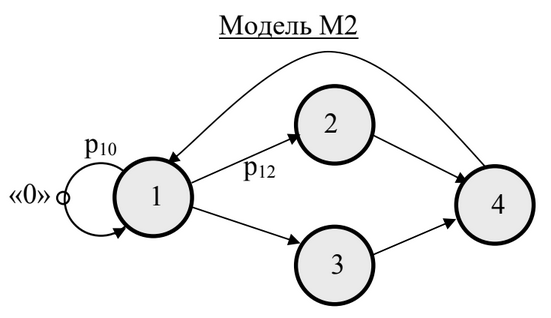
\includegraphics[width=0.5\linewidth]{m2.png}
  \caption{Тип модели M2 в соответствии с вариантом}
\end{figure}

\newpage

\section{Описание моделей}

\subsection{Схема модели замкнутой сети массового обслуживания}

\begin{figure}[h]
  \centering{}
  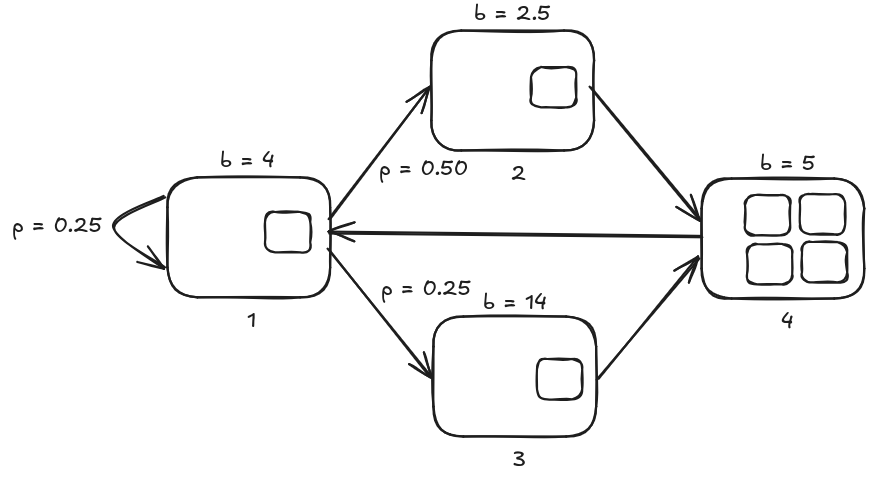
\includegraphics[width=0.5\linewidth]{m2draw.png}
  \caption{Модель замкнутой сети массового обслуживания}
\end{figure}

\subsection{GPSS модели замкнутой сети массового обслуживания}

Установим распределение время обработки одного транзакта во втором узле по закону Эрланга второго порядка.

\begin{lstlisting}
t_b1 EQU 4
t_b2 EQU 2.5
t_b3 EQU 14
t_b4 EQU 5

RN_B EQU 533
RN_erl1 EQU 31
RN_erl2 EQU 125

k EQU 2
Erl_k VARIABLE (Exponential (RN_erl1, 0, t_b2 / k)) + (Exponential (RN_erl2, 0, t_b2 / k))

Node_1 STORAGE 1
Node_2 STORAGE 1
Node_3 STORAGE 1
Node_4 STORAGE 4
; Тест русский
GENERATE ,,,1

Label_0 TRANSFER ,Label_1

Label_1 QUEUE 1
  ENTER Node_1
  DEPART 1
  ADVANCE (Exponential(RN_B, 0, t_b1))
  LEAVE Node_1
  TRANSFER .25,,Label_0
  TRANSFER .50,,Label_2
  TRANSFER .25,,Label_3

Label_2 QUEUE 2
  ENTER Node_2
  DEPART 2
  ADVANCE V$Erl_k
  LEAVE Node_2
  TRANSFER ,Label_4

Label_3 QUEUE 3
  ENTER Node_3
  DEPART 3
  ADVANCE (Exponential(RN_B, 0, t_b3))
  LEAVE Node_3
  TRANSFER ,Label_4

Label_4 QUEUE 4
  ENTER Node_4
  DEPART 4
  ADVANCE (Exponential(RN_B, 0, t_b4))
  LEAVE Node_4
  TRANSFER ,Label_1

GENERATE 100000
TERMINATE 1
\end{lstlisting}

\subsection{Определение критического числа заявок}

Для изменения числа заявок необходимо менять аргумент команды \texttt{GENERATE}.

Далее в отчете GPSS World смотрим на число заявок, которые прошли через метку \texttt{Label\_0} и делим это число на время симуляции (аргумент команды \texttt{GENERATE} в конце модели), получая производительность системы.

\begin{table}[h]
  \centering
  \begin{tabular}{|c|c|}\hline
    Количество заявок & Производительности \\\hline
    1                 & 0.02379            \\\hline
    2                 & 0.04012            \\\hline
    5                 & 0.06023            \\\hline
    10                & 0.06266            \\\hline
    20                & 0.06276            \\\hline
    30                & 0.06286            \\\hline
    40                & 0.06296            \\\hline
    50                & 0.06306            \\\hline
    60                & 0.06316            \\\hline
    75                & 0.06331            \\\hline
    80                & 0.06336            \\\hline
    90                & 0.06346            \\\hline
    95                & 0.06351            \\\hline
    97                & 0.06353            \\\hline
    \textbf{100}      & \textbf{0.06356}   \\\hline
    200               & 0.06356            \\\hline
  \end{tabular}
  \caption{Зависимость производительности ЗСеМО от количества заявок}
\end{table}

\begin{figure}[h]
  \centering
  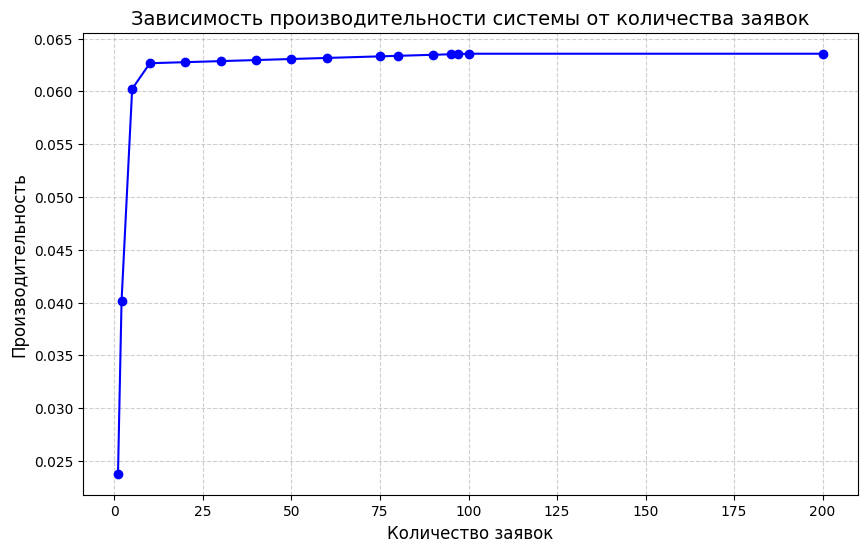
\includegraphics[width=0.5\linewidth]{cm2perfpic.png}
  \caption{Зависимость производительности ЗСеМО от количества заявок}
\end{figure}

\section{Поиск узкого места}

Проанализируем внимательнее отчет GPSS при 100 заявках.

\begin{lstlisting}
              GPSS World Simulation Report - Untitled Model 1.29.1


                   Thursday, December 19, 2024 13:52:41

           START TIME           END TIME  BLOCKS  FACILITIES  STORAGES
                0.000         100000.000    30        0          4


              NAME                       VALUE
          ERL_2                       10007.000
          LABEL_0                         2.000
          LABEL_1                         3.000
          LABEL_2                        11.000
          LABEL_3                        17.000
          LABEL_4                        23.000
          NODE_1                      10008.000
          NODE_2                      10009.000
          NODE_3                      10010.000
          NODE_4                      10011.000
          RN_B                          533.000
          RN_ERL1                        31.000
          RN_ERL2                       125.000
          T_B1                            4.000
          T_B2                            2.500
          T_B3                           14.000
          T_B4                            5.000


 LABEL              LOC  BLOCK TYPE     ENTRY COUNT CURRENT COUNT RETRY
                    1    GENERATE           100             0       0
LABEL_0             2    TRANSFER          6356             0       0
LABEL_1             3    QUEUE            25079            99       0
                    4    ENTER            24980             0       0
                    5    DEPART           24980             0       0
                    6    ADVANCE          24980             1       0
                    7    LEAVE            24979             0       0
                    8    TRANSFER         24979             0       0
                    9    TRANSFER         18723             0       0
                   10    TRANSFER          9293             0       0
LABEL_2            11    QUEUE            16455             0       0
                   12    ENTER            16455             0       0
                   13    DEPART           16455             0       0
                   14    ADVANCE          16455             0       0
                   15    LEAVE            16455             0       0
                   16    TRANSFER         16455             0       0
LABEL_3            17    QUEUE             2268             0       0
                   18    ENTER             2268             0       0
                   19    DEPART            2268             0       0
                   20    ADVANCE           2268             0       0
                   21    LEAVE             2268             0       0
                   22    TRANSFER          2268             0       0
LABEL_4            23    QUEUE            18723             0       0
                   24    ENTER            18723             0       0
                   25    DEPART           18723             0       0
                   26    ADVANCE          18723             0       0
                   27    LEAVE            18723             0       0
                   28    TRANSFER         18723             0       0
                   29    GENERATE             1             0       0
                   30    TERMINATE            1             0       0


QUEUE              MAX CONT. ENTRY ENTRY(0) AVE.CONT. AVE.TIME   AVE.(-0) RETRY
 1                 100   99  25079      1    96.956    386.601    386.616   0
 2                   8    0  16455   9633     0.220      1.337      3.225   0
 3                   6    0   2268   1506     0.148      6.534     19.448   0
 4                   3    0  18723  18512     0.003      0.015      1.361   0


STORAGE            CAP. REM. MIN. MAX.  ENTRIES AVL.  AVE.C. UTIL. RETRY DELAY
 NODE_1              1    0   0     1    24980   1    1.000  1.000    0   99
 NODE_2              1    1   0     1    16455   1    0.417  0.417    0    0
 NODE_3              1    1   0     1     2268   1    0.332  0.332    0    0
 NODE_4              4    4   0     4    18723   1    0.924  0.231    0    0


FEC XN   PRI         BDT      ASSEM  CURRENT  NEXT  PARAMETER    VALUE
    43    0      100004.592     43      6      7
   102    0      200000.000    102      0     29
\end{lstlisting}

Заметим, что утилизация первого узла максимальна - именно он и является узким местом.

Попробуем горизонтально масштабировать данный узел, увеличив количество приборов до 8, и перезапустим симуляцию.

\begin{lstlisting}
STORAGE            CAP. REM. MIN. MAX.  ENTRIES AVL.  AVE.C. UTIL. RETRY DELAY
 NODE_1              8    4   0     8    60814   1    2.439  0.305    0    0
 NODE_2              1    0   0     1    39771   1    1.000  1.000    0   90
 NODE_3              1    0   0     1     5710   1    0.789  0.789    0    2
 NODE_4              4    2   0     4    45479   1    2.275  0.569    0    0
\end{lstlisting}

Теперь производительность системы стала равна 0.15337, что в 2.4 раза больше, чем было (0.06356).

По отчету видим, что утилизация первого узла стала низкой, а теперь мы упираемся во второй узел.

Попробуем докинуть ресурсов и ему, установим на него 4 прибора.

\begin{lstlisting}
STORAGE            CAP. REM. MIN. MAX.  ENTRIES AVL.  AVE.C. UTIL. RETRY DELAY
 NODE_1              8    7   0     8    77985   1    3.142  0.393    0    0
 NODE_2              4    0   0     4    51133   1    1.283  0.321    0    1
 NODE_3              1    0   0     1     7245   1    1.000  1.000    0   91
 NODE_4              4    2   0     4    58373   1    2.917  0.729    0    0
\end{lstlisting}

Обновим 3ий узел, установим 4 прибора и там.

\begin{lstlisting}
STORAGE            CAP. REM. MIN. MAX.  ENTRIES AVL.  AVE.C. UTIL. RETRY DELAY
 NODE_1              8    3   0     8   106546   1    4.254  0.532    0    0
 NODE_2              4    2   0     4    69946   1    1.752  0.438    0    0
 NODE_3              4    4   0     4     9908   1    1.386  0.346    0    0
 NODE_4              4    0   0     4    79763   1    4.000  1.000    0   89
\end{lstlisting}

Заметим, что третий узел не сильно загружен, но обрабатывает запросы медленно. Второй узел работает быстро, но также не очень загружен. Интуитивно кажется, что недогрузка узлов 2 и 3 ведет к перегрузке узла 4. Попробуем уменьшить их производительность, установив по 2 прибора, и 4 прибора на первый узел.

\begin{lstlisting}
STORAGE            CAP. REM. MIN. MAX.  ENTRIES AVL.  AVE.C. UTIL. RETRY DELAY
 NODE_1              4    0   0     4   100022   1    4.000  1.000    0   48
 NODE_2              2    0   0     2    65592   1    1.644  0.822    0    4
 NODE_3              2    0   0     2     9340   1    1.303  0.652    0    2
 NODE_4              4    0   0     4    74894   1    3.744  0.936    0   34
\end{lstlisting}

И снова узел 1 не вывозит. Узел 3 не слишком загружен, но, думаю, это связано с перегрузкой первого узла. Добавим 2 прибора первому узлу.

\begin{lstlisting}
STORAGE            CAP. REM. MIN. MAX.  ENTRIES AVL.  AVE.C. UTIL. RETRY DELAY
 NODE_1              6    2   0     6   106877   1    4.273  0.712    0    0
 NODE_2              2    0   0     2    70164   1    1.757  0.879    0    7
 NODE_3              2    1   0     2     9936   1    1.399  0.699    0    0
 NODE_4              4    0   0     4    80015   1    4.000  1.000    0   82
\end{lstlisting}

Итого мы имеем конфигурацию по приборам (6, 2, 2, 4).

Производительность такой системы составила 0.26866 против 0.15337, то есть мы получили прирост в 1.75 раз. А по сравнению с самой первой версией прирост составил 4.227 раза.

\section{GPPS РСеМО}

\begin{lstlisting}
t_b1 EQU 4
t_b2 EQU 2.5
t_b3 EQU 14
t_b4 EQU 5

t_entry EQU 15.75

RN_B EQU 533
RN_erl1 EQU 31
RN_erl2 EQU 125

k EQU 2
Erl_k VARIABLE (Exponential(RN_erl1, 0, t_b2 / k)) + (Exponential(RN_erl2, 0, t_b2 / k))

Node_1 STORAGE 1
Node_2 STORAGE 1
Node_3 STORAGE 1
Node_4 STORAGE 4

GENERATE (Exponential(RN_B,0,t_entry))

Label_1 QUEUE 1
  ENTER Node_1
  DEPART 1
  ADVANCE (Exponential(RN_B, 0, t_b1))
  LEAVE Node_1
  TRANSFER .25,,Label_0
  TRANSFER .50,,Label_2
  TRANSFER .25,,Label_3

Label_2 QUEUE 2
  ENTER Node_2
  DEPART 2
  ADVANCE V$Erl_k
  LEAVE Node_2
  TRANSFER ,Label_4

Label_3 QUEUE 3
  ENTER Node_3
  DEPART 3
  ADVANCE (Exponential(RN_B, 0, t_b3))
  LEAVE Node_3
  TRANSFER ,Label_4

Label_4 QUEUE 4
  ENTER Node_4
  DEPART 4
  ADVANCE (Exponential(RN_B, 0, t_b4))
  LEAVE Node_4
  TRANSFER ,Label_1

Label_0 TERMINATE 1
\end{lstlisting}

\section{Симуляция PCeMO}

Производительность ЗСеМО составила 0.06356, что эквивалентно потоку заявок раз в 15.73 единиц времени. Разомкнем её и запустим симуляцию.

\begin{lstlisting}
              GPSS World Simulation Report - Untitled Model 1.44.1


                   Thursday, December 19, 2024 15:47:55

           START TIME           END TIME  BLOCKS  FACILITIES  STORAGES
                0.000        1596599.858    28        0          4


              NAME                       VALUE
          ERL_2                       10008.000
          LABEL_0                        28.000
          LABEL_1                         2.000
          LABEL_2                        10.000
          LABEL_3                        16.000
          LABEL_4                        22.000
          NODE_1                      10009.000
          NODE_2                      10010.000
          NODE_3                      10011.000
          NODE_4                      10012.000
          RN_B                          533.000
          RN_ERL1                        31.000
          RN_ERL2                       125.000
          T_B1                            4.000
          T_B2                            2.500
          T_B3                           14.000
          T_B4                            5.000
          T_ENTRY                        15.730


 LABEL              LOC  BLOCK TYPE     ENTRY COUNT CURRENT COUNT RETRY
                    1    GENERATE        101650             0       0
LABEL_1             2    QUEUE           399855          1649       0
                    3    ENTER           398206             1       0
                    4    DEPART          398205             0       0
                    5    ADVANCE         398205             0       0
                    6    LEAVE           398205             0       0
                    7    TRANSFER        398205             0       0
                    8    TRANSFER        298205             0       0
                    9    TRANSFER        148777             0       0
LABEL_2            10    QUEUE           261234             0       0
                   11    ENTER           261234             0       0
                   12    DEPART          261234             0       0
                   13    ADVANCE         261234             0       0
                   14    LEAVE           261234             0       0
                   15    TRANSFER        261234             0       0
LABEL_3            16    QUEUE            36971             0       0
                   17    ENTER            36971             0       0
                   18    DEPART           36971             0       0
                   19    ADVANCE          36971             0       0
                   20    LEAVE            36971             0       0
                   21    TRANSFER         36971             0       0
LABEL_4            22    QUEUE           298205             0       0
                   23    ENTER           298205             0       0
                   24    DEPART          298205             0       0
                   25    ADVANCE         298205             0       0
                   26    LEAVE           298205             0       0
                   27    TRANSFER        298205             0       0
LABEL_0            28    TERMINATE       100000             0       0


QUEUE              MAX CONT. ENTRY ENTRY(0) AVE.CONT. AVE.TIME   AVE.(-0) RETRY
 1                1654 1650 399855    402   856.542   3420.126   3423.568   0
 2                   9    0 261234 154328     0.214      1.306      3.193   0
 3                   8    0  36971  24955     0.158      6.804     20.935   0
 4                   5    0 298205 294849     0.003      0.017      1.471   0


STORAGE            CAP. REM. MIN. MAX.  ENTRIES AVL.  AVE.C. UTIL. RETRY DELAY
 NODE_1              1    0   0     1   398206   1    0.999  0.999    0 1649
 NODE_2              1    1   0     1   261234   1    0.410  0.410    0    0
 NODE_3              1    1   0     1    36971   1    0.327  0.327    0    0
 NODE_4              4    4   0     4   298205   1    0.934  0.233    0    0


CEC XN   PRI          M1      ASSEM  CURRENT  NEXT  PARAMETER    VALUE
 98841    0     1552982.897   98841      3      4


FEC XN   PRI         BDT      ASSEM  CURRENT  NEXT  PARAMETER    VALUE
101651    0     1596602.055   101651      0      1
\end{lstlisting}

\newpage{}

\section{Исследование загрузки узлов от интенсивности потока}

\begin{table}[h]
  \centering
  \begin{tabular}{|c|c|c|c|c|}\hline{}
    Интенсивность & Загрузка N1 & Загрузка N2 & Загрузка N3 & Загрузка N4 \\\hline
    20.00         & 0.797       & 0.327       & 0.261       & 0.186       \\\hline
    19.00         & 0.839       & 0.345       & 0.274       & 0.196       \\\hline
    18.50         & 0.862       & 0.354       & 0.283       & 0.201       \\\hline
    18.00         & 0.886       & 0.364       & 0.291       & 0.208       \\\hline
    17.50         & 0.906       & 0.372       & 0.294       & 0.212       \\\hline
    17.00         & 0.937       & 0.385       & 0.305       & 0.219       \\\hline
    16.50         & 0.970       & 0.398       & 0.316       & 0.227       \\\hline
    16.00         & 0.989       & 0.407       & 0.321       & 0.232       \\\hline
    15.90         & 0.999       & 0.410       & 0.324       & 0.233       \\\hline
    15.80         & 0.999       & 0.411       & 0.324       & 0.234       \\\hline
    15.75         & 0.999       & 0.411       & 0.324       & 0.234       \\\hline
    15.70         & 1.000       & 0.412       & 0.326       & 0.235       \\\hline
    15.60         & 1.000       & 0.411       & 0.326       & 0.234       \\\hline
    15.50         & 1.000       & 0.411       & 0.324       & 0.234       \\\hline
  \end{tabular}
  \caption{Зависимость загруженности PСеМО от интенсивности потока}
\end{table}

\begin{figure}[h]
  \centering
  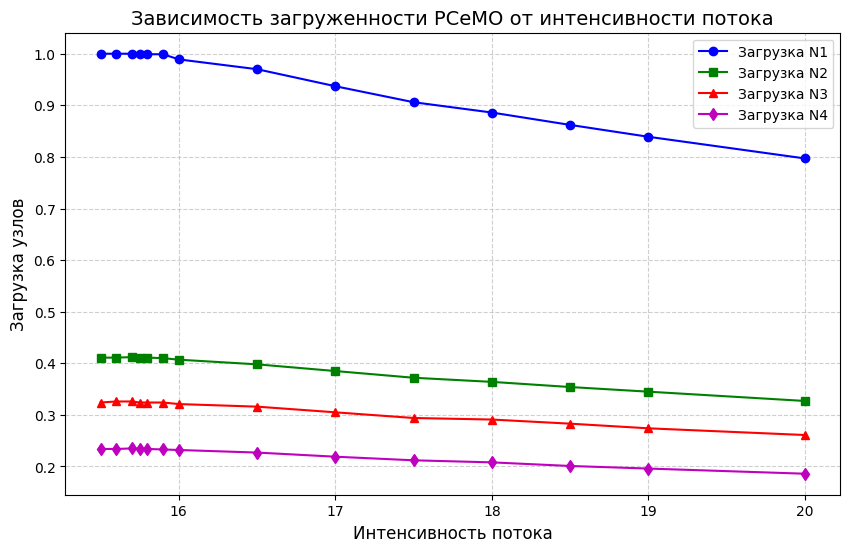
\includegraphics[width=0.5\linewidth]{om2perfpic.png}
  \caption{Зависимость загруженности PСеМО от интенсивности потока}
\end{figure}

\subsection{Оценка влияния коэффициента вариации интервалов времени между заявками на РСеМО}

\begin{table}[h]
  \centering
  \begin{tabular}{|c|c|c|c|c|}\hline{}
                           & Загрузка N1 & Загрузка N2 & Загрузка N3 & Загрузка N4 \\\hline{}
    Детерминированный (17) & 0.938       & 0.385       & 0.308       & 0.220       \\\hline{}
    Простейший (17)        & 0.937       & 0.385       & 0.305       & 0.219       \\\hline{}
  \end{tabular}
  \caption{Влияния коэффициента вариации интервалов времени между заявками на РСеМО}
\end{table}

\newpage{}

\subsection{Оценка влияния коэффициента вариации интервалов времени между заявками на ЗСеМО}

\begin{table}[h]
  \centering
  \begin{tabular}{|c|c|c|c|c|}\hline{}
    Erlang K & Утилизация 1 & Утилизация 2 & Утилизация 3 & Утилизация 4 \\\hline{}
    2        & 0.370        & 0.157        & 0.120        & 0.088        \\\hline{}
    3        & 0.390        & 0.111        & 0.125        & 0.094        \\\hline{}
    4        & 0.401        & 0.085        & 0.130        & 0.096        \\\hline{}
    5        & 0.408        & 0.069        & 0.133        & 0.098        \\\hline{}
    6        & 0.413        & 0.058        & 0.135        & 0.099        \\\hline{}
  \end{tabular}
  \caption{Влияния коэффициента вариации интервалов времени между заявками на ЗСеМО}
\end{table}

\begin{figure}[h]
  \centering{}
  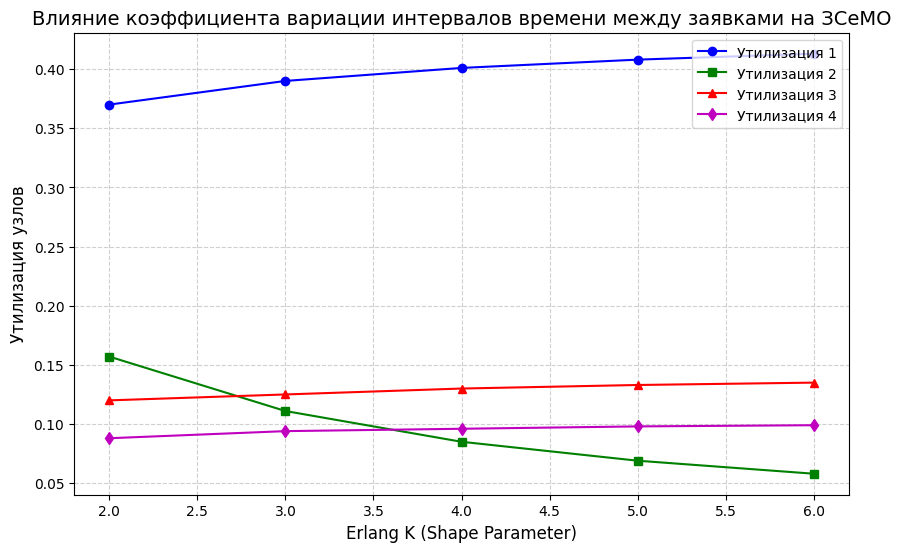
\includegraphics[width=0.5\linewidth]{cm2perfpic2.png}
  \caption{Влияния коэффициента вариации интервалов времени между заявками на ЗСеМО}
\end{figure}

\section{Вывод}

В ЗСМО производительность стабилизируется при достижении критического числа заявок M, определяемого ''узким местом'' сети. Устранение ''узкого места'' в ЗСМО повышает её производительность. В РСМО время пребывания заявок увеличивается с ростом интенсивности входящего потока, а при перегрузке сеть теряет устойчивость. Неэкспоненциальное распределение длительности обслуживания увеличивает время ожидания и пребывания заявок в сети. Сравнение ЗСМО и РСМО показало, что ЗСМО более устойчива к перегрузкам, а РСМО чувствительна к изменению интенсивности потока.

\end{document}
